% Selected immutable publication asset from PR #17; caption adapted from the integration kit.
\begin{figure*}[t]
\centering
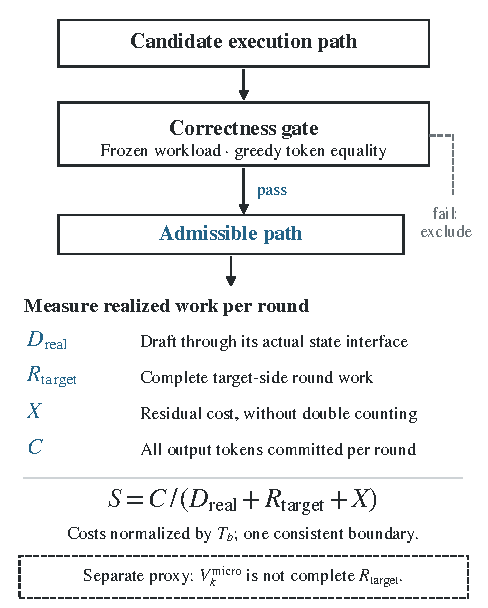
\includegraphics[width=\textwidth]{../figures/pdf/figure1.pdf}
\caption{\textbf{Favorable local signals, divergent realized outcomes}. Near-one-step target batching and favorable isolated drafting do not consistently translate into qualified post-prefill decode gains in the tested cases. The same tested M4 Metal stack exhibits a profitable HumanEval regime and a negative representative-24Q regime in separate frozen studies. RTX batched verification is physically cheap but fails correctness qualification. The 358H NPU has higher isolated median throughput at 8,192 tokens yet reaches only 0.352$\times$ realized speedup. Rows are heterogeneous case summaries, not a hardware ranking or common quantitative axis. M4 micro values describe the shared path in a separate micro study, not independent measurements in each workload. The 8,192-token NPU example is contextualized by all three contexts in Figure~\ref{fig:state}. Headline speedups cover post-prefill decode; Figures~\ref{fig:m4}, \ref{fig:verification}, and~\ref{fig:state} give conditions, uncertainty, and the two measured diagnoses.}
\label{fig:overview}
\end{figure*}
